% Preamble
\documentclass[12pt, a4paper, twoside, romanian]{teza-upb}

% Thesis Settings
\usepackage{soul} % Required for \hl
\setcounter{secnumdepth}{3}
\setcounter{tocdepth}{3}
\usepackage[romanian]{babel}
\usepackage{graphicx}
\usepackage{babel}
\usepackage{color}
\usepackage{graphicx}
\usepackage{lmodern}
\usepackage{microtype}
\usepackage{csquotes}
\usepackage{ragged2e} 
\usepackage{pdfpages}
%\usepackage{cite}
\usepackage[backend=biber,style=numeric-comp,sorting=none,maxnames=99,minnames=99]{biblatex}
\addbibresource{referinte.bib}
\usepackage[justification=centering]{caption}
\usepackage[hidelinks,
  bookmarks,
  bookmarksopen=true,
  pdftitle={Licenta},
  linktocpage]{hyperref}
\usepackage{indentfirst}
\usepackage{titlesec}
\setlength{\parindent}{2em}
\singlespacing

\titleformat{\section}
  {\fontsize{16}{20}\bfseries} % 16pt font size, bold
  {\hspace*{1.25em}\thesection.}              % Section number with a period
  {0.5em}                       % Space between number and title
  {}
  
\titleformat{\subsection}
  {\fontsize{14}{18}\bfseries} % 14pt font size, bold
  {\hspace*{1.5em}\thesubsection.}           % Subsection number with a period
  {0.5em}                     % Space between the number and the title
  {}


%%%%%%%%%%%%%%%%%%%%%%%%%%%%%%%%%%%%%%%%%%%%%%%%%%%%%%%%cod colorat
\usepackage{listings}
\usepackage{color}
\usepackage{enumerate}
\usepackage{verbatim}
 \usepackage{booktabs}
\definecolor{codegreen}{rgb}{0,0.6,0}
\definecolor{codegray}{rgb}{0.5,0.5,0.5}
\definecolor{codepurple}{rgb}{0.58,0,0.82}
\definecolor{backcolour}{rgb}{0.95,0.95,0.92}
\usepackage{algorithm2e}
\lstdefinestyle{mystyle}{
	language=Matlab,
 %   backgroundcolor=\color{backcolour},   
    commentstyle=\color{codegreen},
    keywordstyle=\color{blue},
    numberstyle=\tiny\color{codegray},
    stringstyle=\color{codepurple},
	basicstyle=\ttfamily\scriptsize,
    breakatwhitespace=false,         
    breaklines=true,                 
    captionpos=b,                    
    keepspaces=true,                 
    numbers=left,                    
    numbersep=5pt,                  
    showspaces=false,                
    showstringspaces=false,
    showtabs=false,                  
    tabsize=2
}
 
\lstset{style=mystyle}

\usepackage{enumitem} % Provides customization for lists

% Custom settings for enumerate environment
\setlist[enumerate,1]{label=\alph*), %  lowercase letters with closing parenthesis
                      leftmargin=2cm, % Left margin for the list
                      labelsep=0.2cm, % Space between label and text
                      itemsep=0.0em, % Space between items
                      topsep=0cm, % Space above and below the list
                      parsep=0cm} % Space between paragraphs inside items
\setlist[enumerate,2]{label=\textbf{\textendash}, % Second level: en-dash
                      leftmargin=0.5cm, % Left margin for the list
                      labelsep=0.2cm, % Space between label and text
                      itemsep=0.0em, % Space between items
                      topsep=0cm, % Space above and below the list
                      parsep=0cm} % Space between paragraphs

\setlist[itemize,1]{label=\textbf{\textendash}, %  lowercase letters with closing parenthesis
                      leftmargin=2cm, % Left margin for the list
                      labelsep=0.2cm, % Space between label and text
                      itemsep=0.0em, % Space between items
                      topsep=0cm, % Space above and below the list
                      parsep=0cm} % Space between paragraphs inside items
\setlist[itemize,2]{label=\textbf{\textendash}, % Second level: en-dash
                      leftmargin=0.75cm, % Left margin for the list
                      labelsep=0.2cm, % Space between label and text
                      itemsep=0.0em, % Space between items
                      topsep=0cm, % Space above and below the list
                      parsep=0cm} % Space between paragraphs

\renewcommand{\labelitemi}{\textbf{--}} % First-level bullet


\captionsetup[table]{
    name=Tabelul,
    labelfont=bf,           % Make the label (e.g., "Table 1") bold
    textfont=normal,            % Make the caption text bold
    skip=10pt,              % Add space between the caption and the table
    belowskip=10pt,         % Add space after the caption
    aboveskip=10pt          % Add space before the caption
}

\captionsetup[figure]{
    labelfont=bf,           % Make the label (e.g., "Table 1") bold
    textfont=normal,            % Make the caption text bold
    skip=10pt,              % Add space between the caption and the table
    belowskip=10pt,         % Add space after the caption
    aboveskip=10pt          % Add space before the caption
}



% Format for URLs
\DeclareFieldFormat{url}{Disponibil: \url{#1}}

% Format for DOIs
\DeclareFieldFormat{doi}{DOI: \href{https://doi.org/#1}{#1}}

% Romanian month name fix (avoids abbreviation)
\DefineBibliographyExtras{romanian}{%
  \DeclareFieldFormat{month}{\mkbibmonth{#1}} % Ensures full month names
}

% Remove quotation marks from article, incollection, and inproceedings titles

% Ensure journal and book titles are displayed correctly
\DeclareFieldFormat[article,incollection,inproceedings]{title}{\mkbibquote{#1}}

% Ensure books display correctly with emphasized titles
\DeclareFieldFormat[book]{title}{\mkbibemph{#1}}
\DefineBibliographyExtras{romanian}{%
  \DeclareFieldFormat{month}{\mkbibmonth{#1}} % Ensures full month names
}


\DeclareBibliographyDriver{unpublished}{%
  \usebibmacro{bibindex}%
  \usebibmacro{begentry}%
  \printnames{author}% Print the author (***)
  \setunit{\labelnamepunct}\newblock
  \printfield{title}% Print the title
  \setunit{\labelnamepunct}\newblock
  \printfield{month}% Print the title
  \setunit{\addspace}
  \printfield{year}% Print the title
  \setunit{\adddotspace}\newblock
  \printtext{[Online]}% Add [Online]
  \setunit{\labelnamepunct}\newblock
  \printfield{doi}
  \printfield{note}
  \usebibmacro{finentry}}
  


  \DeclareBibliographyDriver{misc}{%
  \usebibmacro{bibindex}%
  \usebibmacro{begentry}%
  \printnames{author}% Print the author (***)
  \setunit{\labelnamepunct}\newblock
  \printfield{title}% Print the title
  \setunit{\labelnamepunct}\newblock
  \printfield{howpublished}
  \setunit{\adddotspace}\newblock
  \printtext{[Online]}% Add [Online]
  \setunit{\addspace}
  \printfield{url}
  \printfield{note}
  \usebibmacro{finentry}}

  \DeclareBibliographyDriver{incollection}{%
  \usebibmacro{bibindex}%
  \usebibmacro{begentry}%
  \printnames{author}% Print the authors
  \setunit{\labelnamepunct}\newblock
  \printfield{title}% Print the title
  \setunit{\addcomma\space}% Add a comma and space
  \printtext{în }% Add "în" before editor
  \printnames{editor}% Print the editors
  \printtext{ (Eds.)}% Add "(Eds.)"
  \setunit{\addspace}
  \printfield{booktitle}% Print the booktitle
  \setunit{\addspace}
  \printfield{series}% Print the series name
  \setunit{\addcomma\space}
  \printfield{volume}% Print the volume
  \setunit{\addcomma\space}
  \printlist{publisher}% Print the publisher
  \setunit{\addcomma\space}
  \printlist{location}% Print the address
  \setunit{\addcomma\space}
  \printfield{pages}% Print the pages
  \setunit{\addcomma\space}
  \printfield{month}% Print the month
  \setunit{\addspace}
  \printfield{year}% Print the year
  \usebibmacro{finentry}}

  \DeclareBibliographyDriver{inproceedings}{%
  \usebibmacro{bibindex}%
  \usebibmacro{begentry}%
  \printnames{author}% Print the authors
  \setunit{\labelnamepunct}\newblock
  \printfield{title}% Print the title
  \setunit{\addcomma\space}% Add a comma and space
  \printfield{booktitle}% Print the booktitle
  \setunit{\addspace}
  \printfield{series}% Print the series name
  \setunit{\addcomma\space}
  \printfield{volume}% Print the volume
  \setunit{\addcomma\space}
  \printlist{publisher}% Print the publisher
  \setunit{\addcomma\space}
  \printlist{location}% Print the address
  \setunit{\addcomma\space}
  \printfield{pages}% Print the pages
  \setunit{\addcomma\space}
  \printfield{month}% Print the month
  \setunit{\addspace}
  \printfield{year}% Print the year
  \usebibmacro{finentry}}

\DeclareBibliographyDriver{article}{%
  \usebibmacro{bibindex}%
  \usebibmacro{begentry}%
  \printnames{author}% Print the authors
  \setunit{\labelnamepunct}\newblock
  \printfield{title}% Print the title
  \setunit{\addcomma\space}% Add a comma and space
  \printfield{journaltitle}% Print the booktitle
  \setunit{\addcomma\space}
  \printtext{vol.}
  \printfield{volume}% Print the volume
  \setunit{\addcomma\space}
  \printtext{nr.}
  \printfield{number}
  \setunit{\addcomma\space}
  \printlist{publisher}% Print the publisher
  \setunit{\addcomma\space}
  \printlist{location}% Print the address
  \setunit{\addcomma\space}
  \printfield{pages}% Print the pages
  \setunit{\addcomma\space}
  \printfield{month}% Print the month
  \setunit{\addspace}
  \printfield{year}% Print the year
  \usebibmacro{finentry}}

\renewcommand*{\finalnamedelim}{\addcomma\space} % Changes "și" to "and" and adds commas
\renewcommand*{\multinamedelim}{\addcomma\space}          % Adds commas between multiple authors

\begin{document}
% First Page
\author{\hl{Prenume NUME}}
\title{\hl{\textit{Titlul temei lucrării de disertație}}}
\facultatea{Facultatea de Electronică, Telecomunicații și Tehnologia Informației}
%\tiplucrare{licență}
\tiplucrare{dizertație}
\submissiondate{\hl{data}}
\campus{Leu} 
\program{BIOSINF}
%\titlulobtinut{Inginer}
\titlulobtinut{Master}
\advisor{\hl{Titlu Prenume NUME}} 

\beforepreface

% Lista Tabelelor
\listoftables

% Lista Figurilor
\listoffigures

\cleardoublepage

% Lista abrevierilor
\abbreviations{
CNN	& \textit{Convolutional Neural Network} (lb. en.; rețea neurală convoluțională)\\
IA	& Inteligență artificială\\
MFCC & \textit{Mel-frequency Cepstral Coefficient} (lb. en.; coeficient Mel-cepstral)\\
RODeCAR & \textit{Romanian Deva Criminal Investigation Audio Recordings} (set de date) 
}

\cleardoublepage
%\preface{}
\afterpreface 

% Setari probabil pentru continutul capitolelor.
\pagenumbering{arabic}
\pagestyle{plain}
\setcounter{page}{1}

% Continutul Capitolelor

\chapter{FORMA DE PREZENTARE.\\ STRUCTURA LUCRĂRII}

Materialele se prezintă editate cu toate semnele diacritice din limba română, cu figurile și tabelele incluse în text. Se va folosi fontul Times New Roman, mărime 12 pt. Formatul paginii va fi A4; margini: 2.5 cm – sus, jos, stânga, dreapta.

Titlurile capitolelor se vor scrie centrat, cu majuscule și vor fi precedate de un simbol numeric, începând cu cifra 1, urmată de un punct; pentru subtitluri, vor urma și alte cifre, despărțite între ele prin puncte, în funcție de gradul titlului subordonat (ex.: 1. CAPITOL; 1.1. Subcapitol; 1.1.1. Subcapitol secundar). Nu se vor utiliza mai mult de 3 grade de titluri (capitole, subcapitole, subcapitole secundare).

Fonturi și aliniere pentru titluri:
\begin{itemize}
	\item titlul capitolului: font 18 pt, \textbf{bold}, majuscule, centrat;
	\item titluri subcapitole: font 16 pt, \textbf{bold}, \textit{Sentence case}, aliniat la stânga, tab de 1 cm;
	\item titluri subcapitole secundare: font 14 pt, \textbf{bold}, \textit{Sentence case}, aliniat la stânga, tab de 1 cm.
\end{itemize}

 Pentru spațierea titlurilor, se vor lăsa rânduri libere (font 12 pt) astfel:
 \begin{itemize}
	\item pentru titlul capitolului (pe prima pagină): 5 rânduri deasupra, 3 rânduri dedesubt;
	\item pentru subtitluri: 2 rânduri deasupra, 1 rând dedesubt;
	\item pentru subtitlurile secundare: 1 rând deasupra, 1 rând dedesubt.
\end{itemize}

După titluri (capitole, subcapitole etc.) nu se pune punct; excepție fac titlurile urmate de subtitluri (ex.: „Introducere. Aspecte fundamentale în ...”).

Un subtitlu trebuie să fie urmat întotdeauna de cel puțin 2 rânduri de text pe aceeași pagină; dacă nu a rămas suficient spațiu, se va deplasa totul pe pagina următoare. \\

Textul propriu-zis se va scrie cu font Times New Roman, spațiere 1.15\textbf{--}1.2 rânduri, mărime 12 pt, \textit{Justified}, tab de 1 cm la primul rând al paragrafului.

În text, la sfârșit de rând, dacă este cazul, se face despărțirea cuvintelor în silabe, pentru a nu lăsa spații albe, neuniforme între cuvinte.

Se recomandă să nu se folosească pe parcursul lucrării multe tipuri de simboluri pentru enumerări (\textit{Bullets}); enumerările se vor scrie cu un tab de 1.5 cm, apoi cele imbricate cu tab de 2.25 cm, respectiv 3 cm. De asemenea, se recomandă folosirea cratimei (-) pentru cuvintele compuse și a liniei lungi (\textbf{--}, \textit{En dash}) pentru enumerări sau explicații.

Se recomandă să nu existe în partea de jos a paginii un paragraf nou cu mai puțin de 2 rânduri; același lucru pentru un paragraf care se termină la începutul paginii următoare.

Structura lucrării trebuie să cuprindă:
\begin{itemize}
    \item pagini inițiale (înaintea corpului lucrării):
    \begin{itemize}
        \item pagină de titlu (pagină goală pe verso) \textbf{--} se vor înlocui secțiunile marcate cu galben din prezentul ghid; dacă titlul ocupă 1 rând, se vor lăsa libere rândurile de deasupra și de dedesubt; dacă titlul ocupă 2 rânduri, se va lăsa liber rândul de dedesubt; titlurile coordonatorilor științifici pot fi Prof. dr. ing., Conf. dr. ing., Ș.L. dr. ing. sau Dr. ing. / Ing. (externi UPB);
	\item Anexa 2 \textbf{--} se va descărca de pe site-ul de absolvire și se va include în continuare, conform specificației prezentului ghid;
	\item declarație de onestitate academică (pagină goală pe verso) – se vor înlocui secțiunile marcate cu galben din prezentul ghid;
	\item cuprins \textbf{--} se vor înlocui secțiunile marcate cu galben din prezentul ghid;
	\item lista tabelelor, lista figurilor și lista abrevierilor (în această ordine) \textbf{--} se vor înlocui secțiunile marcate cu galben din prezentul ghid;
    \end{itemize}
    \item corpul lucrării (capitole numerotate):
	\begin{itemize}
	    \item introducere (capitolul 1) \textbf{--} domeniul abordat, descrierea problemei, evidențierea oportunităților de îmbunătățire, structura concretă a lucrării;
	\item următoarele capitole propriu-zise ale lucrării (capitolele 2, 3, ...) \textbf{--} acestea pot fi, spre exemplu, un capitol de trecere în revistă a stării artei și de detaliere concisă a noțiunilor teoretice (tehnici de analiză și prelucrare de semnale, modele de învățare automată etc.) utilizate în cadrul lucrării (capitolul 2), unul sau două capitole de definire și detaliere a unui sistem sau a unor tehnici originale propuse (capitolul 3 / capitolele 3-4) și un capitol de prezentare a seturilor de date utilizate, a metodologiei experimentale și a rezultatelor obținute, împreună cu interpretarea acestora (capitolul 4/5);
	\item concluzii (ultimul capitol) \textbf{--} concluzii generale, contribuții originale, dezvoltări ulterioare;
    \end{itemize}
    \item bibliografie.\\
\end{itemize}

Lucrarea de disertație se tipărește față-verso.

Cuprinsul și listele tabelelor, figurilor și abrevierilor vor fi numerotate folosind cifre romane (prima pagină a cuprinsului: pagina v). Capitolele propriu-zise și bibliografia vor fi numerotate folosind cifre arabe (prima pagină a primului capitol: pagina 1).

Toate secțiunile (cuprinsul, listele tabelelor, figurilor și abrevierilor, capitolele și bibliografia) trebuie să înceapă pe pagină \textbf{nouă}, \textbf{dreaptă} (deci impară); dacă este necesar, se vor lăsa pagini goale și nenumerotate, după caz (exemplificat în prezentul ghid).

Se recomandă ca introducerea (capitolul 1) să cuprindă 2\textbf{--}4 pagini, concluziile (ultimul capitol) să cuprindă 2\textbf{--}4 pagini, iar restul capitolelor (capitolul 2, 3, ...) să fie proporționale. De asemenea, subcapitolele și subcapitolele secundare trebuie să fie și ele proporționale. Nu se justifică să existe capitole de 3 pagini față de capitole de 20 de pagini, la fel cum nu se justifică subcapitole mai scurte de 1 pagină sau subcapitole secundare mai scurte de jumătate de pagină.

Se recomandă ca lucrarea de disertație să aibă \textbf{între 60 și 80 de pagini}.



%\begin{figure}[h]
%    \centering
%    \includegraphics[width=0.5\textwidth]{figuri/punguta.jpg}
%    \caption{Exemplu de figură.}
%    \label{fig:exemplu}
%\end{figure}


%Figura \ref{fig:exemplu} reprezintă un exemplu.



\chapter{NOTAȚII MATEMATICE. REGULI ORTOGRAFICE}

\section{Mărimi și unități de măsură}

În cadrul aceleiași lucrări, nu se admite ca o mărime să fie notată cu mai multe simboluri. De asemenea, se va evita pe cât posibil ca mărimi diferite să fie notate cu același simbol.

Unitățile de măsură folosite trebuie să aparțină Sistemului Internațional de Unități de Măsură (SI) și, tot conform acestuia, se vor adopta simbolurile lor.


\section{Notații folosite în formulele matematice}

\subsection{Reguli generale}

Simbolul pentru scădere (minus) trebuie să fie linia lungă (\textbf{--}, \textit{En dash}), nu cratima (-).

Valorile numerice (mărimi, indici, exponenți etc.) se vor scrie drept (nu \textbf{bold}/\textit{italic}).

Mărimile se vor nota cu simboluri scrise \textit{italic} (indiferent dacă se folosesc litere ale alfabetului latin sau litere grecești), iar valoarea numerică a mărimii și unitatea de măsură se vor scrie drept, cu spațiu între ele – ex.: $f_e$ = 16 kHz, $\sigma^2$ = 1.

În cazul utilizării unei unități de măsură separat de o valoare numerică (ex.: etichetarea axelor figurilor), unitatea de măsură se va scrie între paranteze drepte; ex.: $f$ [Hz], $|S(e^{j\omega})|$ [dB].

Mărimile de natură vectorială se vor scrie \textbf{bold} și drept; vectorii vor fi scriși cu minuscule, matricele cu majuscule – ex.: \textbf{x}\textsubscript{\textit{n}} = [\textit{F}\textsubscript{0}; \textit{F}\textsubscript{1}; ...; \textit{F}\textsubscript{\textit{D}-1}], \textbf{X} = [\textbf{x}\textsubscript{0}, \textbf{x}\textsubscript{1}, ..., \textbf{x}\textsubscript{\textit{N}-1}].

Ecuațiile vor fi centrate, pe rând nou. Între ecuații și text se va lăsa o distanță de 1 rând liber (12 pt) deasupra și dedesubtul lor. Explicațiile notațiilor dintr-o ecuație se recomandă să fie scrise în paragraful în care este referită ecuația.

Ecuațiile vor fi numerotate în continuare, pe capitole (ex.: (\ref{Eq_freq}) ). Numărul curent al ecuației se va scrie între paranteze rotunde, plasat în dreapta, la marginea formatului textului.

Toate ecuațiile se vor numerota și trebuie referite în text înainte de scrierea acestora.

\subsection{Alte reguli}

	Pentru formatul fonturilor:
 \begin{enumerate}
     \item se vor mai scrie \textit{italic}:
     \begin{enumerate}
         \item variabile \textbf{--} ex.: \textit{x}, \textit{y}, \textit{z};
         \item funcții oarecare \textbf{--} ex.: \textit{f}, \textit{g}, \textit{f}(x), \textit{v}(n);
         \item indici/exponenți care reprezintă la rândul lor simbolul unei mărimi \textbf{--} ex.: $e^{j\omega}$;
         \item cuvinte în limbi străine care \textbf{nu} sunt incluse în DEX \textbf{--} ex.: funcție \textit{kernel}; pe cât posibil, însă, \textbf{se va încerca traducerea corespunzătoare a acestora}.\\
     \end{enumerate} 
     \item se vor mai scrie drept:
     \begin{enumerate}
         \item funcțiile matematice consacrate \textbf{--} ex.: funcții trigonometrice (sin, cos, tanh etc.), funcții logaritm (log, lg, ln);
	\item notația d pentru derivare  \( \displaystyle \left( \frac{\textnormal{d}v}{\textnormal{d}t} \right) \) și simbolul pentru derivare parțială ($\partial$);
	\item simbolurile pentru limită (lim), constant (ct.), integrală ($\int$), unitatea imaginară (i sau j), constante (e, $\pi$ etc.);
	\item indici (inferiori sau superiori) care provin din prescurtări – ex.: min, max, inf, sup etc.\\
     \end{enumerate}
 \end{enumerate}

În finalul acestui capitol este ilustrat un exemplu prin (\ref{Eq_freq}), aceasta fiind condiția lui Nyquist asociată teoremei eșantionării, unde $f_e$ este frecvența de eșantionare, iar $f_m$ reprezintă frecvența maximă din componența semnalului.

\begin{equation}
    f_e > 2 \cdot f_m
    \label{Eq_freq}
\end{equation}

\section{Reguli ortografice}

Pauza \textbf{nu se folosește înainte, ci după} punct (.), virgulă (,), două puncte (:), punct şi virgulă(;), semnul exclamării (!), semnul întrebării (?).
 
În cazul citatelor unde se folosesc ghilimele, pauza se folosește \textbf{înaintea} ghilimelelor de la începutul citatului (nu între ghilimele și primul cuvânt al citatului), iar în cazul ghilimelelor de la sfârșitul citatului pauza se folosește \textbf{după} ghilimele. Aceeași regulă este valabilă în cazul parantezelor.\\

Pentru cuvintele în limbi străine care \textbf{nu} sunt incluse în DEX, sufixul formei de plural și/sau articolul hotărât se separă de cuvânt prin cratimă \textbf{--} ex.: \textit{kernel}-uri, \textit{transformer}-ele.

Pentru cuvintele în limbi străine care au fost incluse în DEX (fără a li se adapta forma), sufixul formei de plural și/sau articolul hotărât \textbf{nu} se separă prin cratimă dacă forma de singular a cuvântului se termină cu o \textbf{consoană} \textbf{--} ex.: patternuri, kurtosisul.




\chapter{TABELE ȘI FIGURI}

\section{Tabele}

Se vor evita tabelele mari; nu este permis să depășească formatul paginii.

Tabelele din lucrare trebuie să aibă o prezentare unitară. Fiecare tabel trebuie să fie numerotat și să aibă o legendă (titlu / descriere sumară). Legenda tabelului se va scrie \textbf{bold}, drept, centrat, deasupra tabelului \textbf{--} ex.: \textbf{Tabelul 3.1.} Rezultate obținute (validare).

Între un paragraf și legenda unui tabel se lasă un rând liber (12 pt); la fel între tabel și paragraful următor. Între legendă și tabel se lasă un rând liber (12 pt).

Dacă tabelul este mai mare, se poate folosi în interior scrierea la un rând, eventual și cu font mai mic de 12. Prima linie a tabelului (și/sau prima coloană, după caz) se va scrie \textbf{bold}.

În tabele se vor folosi aceleași fonturi și reguli de editare ca pentru ecuații.

Trimiterile din text la tabele se vor face scriind drept cuvântul „Tabelul” urmat de numărul acestuia.

Dacă există tabele care cuprind note, acestea se vor scrie imediat după tabel, nu la piciorul paginii și nici în corpul tabelului.

Dacă un tabel ar fi prea lung astfel încât ar depăși o pagină întreagă, atunci se va despărți, într-un mod corespunzător, în două (sau mai multe) tabele distincte.

Tabelele vor fi numerotate în continuare, pe capitole – ex.: 2.1, 2.2, ..., 3.1, 3.2, ...

Toate tabelele se vor numerota și trebuie referite în text \textbf{înainte} de prezentarea acestora. \\

În finalul acestui subcapitol este ilustrat un exemplu de tabel, acesta fiind Tabelul \ref{comp}, unde UA și WA reprezintă acuratețea neponderată, respectiv ponderată.

\vfill

\begin{table}
\centering
\caption{Rezultate obținute (validare).}
\label{comp}
\begin{tabular}{|l|r|r|}
\hline
\textbf{Model}                    & \textbf{UA [\%]} & \textbf{WA [\%]}  \\\hline
DNN (3 straturi
  ascunse, ReLU)  & 66.5             & 70.2              \\\hline
DNN (3 straturi
  ascunse, tanh)  & 66.8             & 71.0              \\\hline
CNN (5 straturi
  convoluționale) & 75.4             & 79.3              \\\hline
CNN (8 straturi
  convoluționale) & 54.2             & 58.1              \\\hline
ResNet50                          & 70.6             & 73.9              \\\hline
ResNet50V2                        & 72.3             & 75.7             \\\hline
\end{tabular}
\end{table}

\section{Figuri}

Figurile vor fi incluse în text și pot fi alb-negru sau color, cu un contrast foarte bun între nuanțele de gri sau culori, fără să depășească formatul paginii.

Fiecare figură trebuie numerotată și să aibă o legendă (titlu / descriere sumară). Legenda figurii se va scrie \textbf{bold}, drept, centrat, sub figură – ex.: \textbf{Figura 3.1.} Exemplu de evoluție a funcției cost pentru antrenare și pentru validare. Este marcat punctul în care modelul începe să manifeste supraantrenare.

Între un paragraf și o figura se lasă un rând liber (12 pt); la fel între legenda figurii și paragraful următor. Între figură și legendă se lasă un rând liber (12 pt).

În figuri se vor folosi aceleași fonturi și reguli de editare ca pentru formule.

Trimiterile din text la o anumită figură sau la mai multe figuri se vor face scriind drept cuvântul „Figura”/„Figurile” urmat de numerele acestora – ex.: Figura 3.1, Figurile 4.1-4.2.

Figurile se vor poziționa centrat, pe cât posibil în partea de sus sau de jos a paginii, dar \textbf{după} locul în care sunt referite prima oară în text.
	
 În cazul diagramelor care reprezintă variații calitative, pe axele de coordonate (la capete și în afara desenului) se vor indica doar simbolurile mărimilor în cauză; în schimb, în cazul diagramelor cantitative, axele de coordonate vor cuprinde valorile și unitățile de măsură corespunzătoare mărimilor ce variază.
	
 \textbf{Se recomandă insistent} să nu rămână spații goale mari pe pagină, înainte de o figură care s-ar poziționa la începutul paginii următoare.
	
 Figurile vor fi numerotate în continuare, pe capitole – ex.: 2.1, 2.2, ..., 3.1, 3.2, ...
	
 Toate figurile se vor numerota și trebuie referite în text \textbf{înainte} de prezentarea acestora.\\

	
În finalul acestui subcapitol este ilustrat un exemplu de figură, aceasta fiind Figura \ref{fig:exemplu}.


\begin{figure}[h]
\centering
    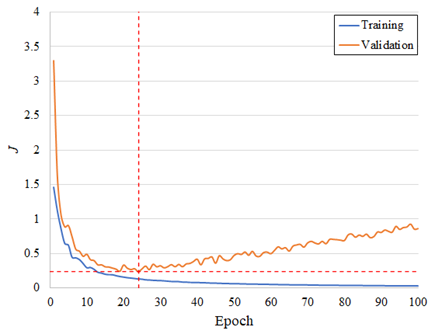
\includegraphics[width=0.7\textwidth]{../png/Figura1}
    \caption{Exemplu de evoluție a funcției cost pentru antrenare și pentru validare. Este marcat punctul în care modelul începe să manifeste supraantrenare.}
    \label{fig:exemplu}
\end{figure}

\chapter{BIBLIOGRAFIE. REGULI DE CITARE}

\section{Bibliografie}

Lucrările se scriu în cadrul referințelor bibliografice în ordinea alfabetică a numelor primilor autori, numerotându-se cu cifre arabe între paranteze drepte. Titlul lucrării se scrie în referința bibliografică exact cum este tipărit în publicația citată.

Mai jos sunt prezentate câteva exemple de scriere a referințelor bibliografice – primul exemplu pentru cărți \cite{Burileanu2022}, al doilea pentru capitole de cărți \cite{Kao2020}, al treilea pentru lucrări de conferință \cite{Zhang2021}, al patrulea pentru articole (în jurnale/reviste) \cite{Yi2022}, iar ultimele două pentru resurse disponibile online \cite{Zeiler2012,MATLAB2025}.

Trimiterile din text la bibliografie se fac scriind drept, între paranteze drepte, numărul de ordine al lucrării/lucrărilor – ex.: \cite{Burileanu2022}; \cite{Kao2020,Zeiler2012}; \cite{Zhang2021,Yi2022,Zeiler2012,MATLAB2025}.

\printbibliography[heading=none]

Wikipedia \textbf{nu} este o resursă bibliografică acceptabilă.

\newpage


\section{Reguli de citare}

\textbf{Este foarte puternic recomandat} să nu se preia ca atare fragmente de text din alte lucrări, ci să fie reformulate ideile, în particular într-un mod sintetic și cu accent pe relevanța lor pentru lucrarea de disertație.

Dacă, totuși, se preia ca atare un fragment de text din altă lucrare, atunci este \textbf{obligatoriu} ca acesta să fie scris între \textbf{ghilimele} și să includă \textbf{referința bibliografică} – ex.: „Modelul sursă-filtru exprimă faptul că efectele compuse ale tractului vocal și radiației buzelor sunt reprezentate printr-un filtru digital cu parametri lent variabili în timp.” [7].\\

\textbf{Este foarte puternic recomandat} ca toate tabelele și figurile prezentate în lucrarea de disertație să fie \textbf{originale}.

Dacă, totuși, se preia ca atare un tabel sau o figură din altă lucrare, atunci este \textbf{obligatoriu} ca legenda acestuia să includă \textbf{referința bibliografică} \textbf{--} ex.: \textbf{Figura 4.5.} Arhitectura rețelei AlexNet [8].

Dacă se preia un tabel sau o figură din altă lucrare și se fac doar modificări minore, atunci este \textbf{obligatoriu} ca legenda acestuia să includă \textbf{referința bibliografică} după care au fost făcute modificările \textbf{--} ex.: \textbf{Figura 4.5.} Exemplu de rețea neurală convoluțională (după [8]).

Evident, în lucrarea de disertație, tabelul/figura va fi numerotat(ă) conform regulilor din capitolul 3 din prezentul ghid; nu este relevantă numerotarea tabelului/figurii din lucrarea originală.

\section{Asumarea proprietății intelectuale (\textit{copyright})}
Implicit, proprietatea intelectuală asupra lucrării (\textit{copyright}-ul) aparține UNSTPB.
În cazul în care absolventul dorește să pretindă drepturile de proprietate intelectuală
pentru propria persoană sau pentru o companie comercială (în cazul în care a existat o astfel
de colaborare), absolventul trebuie să contacteze \textbf{în timp util} coordonatorul științific.





% Bibliografia
%\bibliographystyle{unsrt}
%\bibliography{referinte}

\printbibliography[heading=bibintoc,title={BIBLIOGRAFIE}]

% Nu stiu ce este acest \appendix - DE INTREBAT
\appendix
%\include{Appendix1}
\appendix
\chapter{Source codes}
\noindent
The source codes for this project are available online on \\
\href{https://gitlab.com/adanila/disertatie-deep-fake}{GitLab at https://gitlab.com/adanila/disertatie-deep-fake}

\end{document}
